\documentclass[11pt]{article}
\usepackage[T1]{fontenc}
\usepackage[margin=0.93in]{geometry}
\usepackage{amsmath,amssymb,amsthm,mathtools,microtype,graphicx,enumitem}
\usepackage[colorlinks=true,urlcolor=blue,citecolor=blue,linkcolor=blue]{hyperref}
\newtheorem{theorem}{Theorem}
\newtheorem{lemma}[theorem]{Lemma}
\newtheorem{corollary}[theorem]{Corollary}
\newcommand{\R}{\mathbb R}
\newcommand{\F}{\mathcal F}
\newcommand{\supp}{\operatorname{supp}}
\newcommand{\D}{\mathsf D}
\newcommand{\J}{\mathsf J}
\newcommand{\norm}[1]{\lVert #1\rVert}

\title{The compact-support fractional Poincar\'e inequality at every
\(1\leq p<\infty\)}
\author{Full-resolution packet for \texttt{fa\_banach\_001}}
\date{12 August 2026}

\begin{document}
\maketitle

\noindent\textbf{Status.}
Candidate full resolution of Question~7.4 in arXiv:2001.06210, subject to
human review.  The range \(1<p<\infty\) appeared later in the literature.
The proof below also covers the omitted endpoint \(p=1\), answers the
authors' lower-order-derivative question for every \(0\leq t\leq s\), and
gives the requested dependence on a classical Poincar\'e constant when
\(1<p<\infty\) and \(s\geq1\).

\section*{Source question}

G.~Covi, K.~M\"onkk\"onen, and J.~Railo,
\emph{Unique continuation property and Poincar\'e inequality for higher
order fractional Laplacians with applications in inverse problems},
arXiv:2001.06210 \cite{source}.  Question~7.4 on PDF page~32 asks whether,
for \(s\geq0\), \(1\leq p<\infty\), compact \(K\subset\R^n\), and
\(u\in H^{s,p}(\R^n)\) supported in \(K\),
\begin{equation}\label{eq:source}
  \norm{u}_{L^p(\R^n)}
  \leq C(n,K,s,p)\norm{(-\Delta)^{s/2}u}_{L^p(\R^n)}.
\end{equation}
The following paragraph asks whether \(u\) can be replaced by
\((-\Delta)^{t/2}u\), \(0\leq t\leq s\), and whether the constant can be
expressed using a classical Poincar\'e constant for \(s\geq1\).

\begin{center}

\includegraphics[width=0.96\linewidth]{figures/open_problem_crop.png}
\end{center}

\section*{Definitions and proof intuition}

Write
\[
 \D^r=(-\Delta)^{r/2},\qquad
 \J^r=(I-\Delta)^{r/2},\qquad
 \widehat{\D^r u}(\xi)=|\xi|^r\widehat u(\xi).
\]
The Bessel-potential space \(H^{s,p}(\R^n)\) consists of
\(u=\J^{-s}f\) with \(f\in L^p\), with norm
\(\norm{u}_{H^{s,p}}=\norm{\J^su}_p\).

The usual Mikhlin and Riesz-transform arguments are not \(L^1\)-bounded.
We instead use symbols whose inverse Fourier transforms are finite
measures.  They give the endpoint graph estimate
\[
 \norm{\J^su}_p\lesssim \norm u_p+\norm{\D^su}_p
 \quad(1\leq p\leq\infty).
\]
If the Poincar\'e estimate failed, normalized counterexamples would be
bounded in \(H^{s,p}\).  Fixed compact support and the \(L^1\) Bessel
kernel make this family precompact in \(L^p\), even at \(p=1\).  A limit
would have Fourier transform supported at the origin, hence be a
polynomial; no nonzero polynomial lies in finite \(L^p\).

\section*{Endpoint-safe multiplier lemma}

Let \(\mathcal W(\R^n)\) be the Wiener algebra of Fourier transforms of
finite complex Borel measures.  If \(m=\widehat\mu\in\mathcal W\), then
\(f\mapsto\F^{-1}(m\widehat f)=\mu*f\) is bounded on every \(L^p\),
\(1\leq p\leq\infty\).

\begin{lemma}[Dyadic Wiener criterion]\label{lem:wiener}
Let \(N>n\), and let \(a\in C^N(\R^n\setminus\{0\})\).  Suppose that for
all \(|\alpha|\leq N\),
\[
 |\partial^\alpha a(\xi)|\leq C_\alpha |\xi|^{\rho-|\alpha|}
 \quad(0<|\xi|\leq1),\qquad
 |\partial^\alpha a(\xi)|\leq C_\alpha |\xi|^{-\sigma-|\alpha|}
 \quad(|\xi|\geq1)
\]
for some \(\rho,\sigma>0\).  Then
\(\F^{-1}a\in L^1(\R^n)\), hence \(a\in\mathcal W(\R^n)\).
\end{lemma}

\begin{proof}
Choose a smooth annular dyadic partition
\(1=\sum_{j\in\mathbb Z}\psi(2^{-j}\xi)\) away from zero and set
\(a_j(\xi)=a(\xi)\psi(2^{-j}\xi)\).  Rescaling to a fixed annulus and
integrating by parts \(N>n\) times gives
\[
 \norm{\F^{-1}a_j}_1
 \leq C\max_{|\alpha|\leq N}
 2^{j|\alpha|}\norm{\partial^\alpha a}_{L^\infty(|\xi|\asymp2^j)}.
\]
The bound is \(O(2^{j\rho})\) for \(j\leq0\) and
\(O(2^{-j\sigma})\) for \(j\geq0\).  Both series converge, so
\(\sum_j\F^{-1}a_j\) converges absolutely in \(L^1\).
\end{proof}

\begin{lemma}[The required symbols]\label{lem:symbols}
For \(s>0\), the following symbols belong to \(\mathcal W(\R^n)\):
\begin{align*}
 m_s(\xi)&=\frac{(1+|\xi|^2)^{s/2}}{1+|\xi|^s},
 &b_s(\xi)&=\frac{|\xi|^s}{(1+|\xi|^2)^{s/2}},\\
 a_{s,t}(\xi)&=\frac{|\xi|^t}{1+|\xi|^s},
 &&0\leq t\leq s.
\end{align*}
\end{lemma}

\begin{proof}
The symbol \(m_s-1\) satisfies Lemma~\ref{lem:wiener} at both ends with
positive exponent \(\min\{s,2\}\) (for \(s=2\) it vanishes).  Hence
\(m_s\in\mathcal W\).

Let \(\chi\) be smooth, compactly supported, and one near zero.
The term \(\chi b_s\) has low-frequency exponent \(s\), while
\((1-\chi)(b_s-1)\) has high-frequency decay exponent
\(\min\{s,2\}\).  These terms satisfy Lemma~\ref{lem:wiener}, and
\(b_s=\chi b_s+(1-\chi)+(1-\chi)(b_s-1)\in\mathcal W\).

If \(0<t<s\), then \(a_{s,t}\) has low exponent \(t\) and high decay
exponent \(s-t\), so the criterion applies.  For \(t=0\), write
\(a_{s,0}=\chi+(a_{s,0}-\chi)\); the second term has exponent \(s\) at
both ends.  Finally \(a_{s,s}=1-a_{s,0}\).
\end{proof}

\begin{corollary}[Endpoint graph norm]\label{cor:graph}
For \(s>0\) and \(1\leq p\leq\infty\),
\begin{equation}\label{eq:graph}
 \norm{\J^su}_p\leq C_{n,s}
 \bigl(\norm u_p+\norm{\D^su}_p\bigr).
\end{equation}
Moreover \(\D^s:H^{s,p}\to L^p\) is bounded, including at \(p=1\).
\end{corollary}

\begin{proof}
Use Lemma~\ref{lem:symbols} in the identities
\[
 \widehat{\J^su}=m_s(\widehat u+\widehat{\D^su}),\qquad
 \widehat{\D^su}=b_s\widehat{\J^su}.
\]
\end{proof}

\section*{Full resolution}

\begin{theorem}[All-\(p\) compact-support Poincar\'e inequality]
\label{thm:main}
Let \(K\subset\R^n\) be compact, \(s>0\), and \(1\leq p<\infty\).  There
is \(C=C(n,K,s,p)\) such that every \(u\in H^{s,p}(\R^n)\) with
\(\supp u\subset K\) satisfies
\begin{equation}\label{eq:main}
 \norm u_p\leq C\norm{\D^su}_p.
\end{equation}
More strongly, for every \(0\leq t\leq s\), there is
\(C_t=C(n,K,s,t,p)\) such that
\begin{equation}\label{eq:allt}
 \norm{\D^tu}_p\leq C_t\norm{\D^su}_p.
\end{equation}
For \(s=0\), the source question is the identity with \(C=1\).
\end{theorem}

\begin{proof}
First we prove compactness at the endpoint.  The Bessel kernel
\(G_s=\F^{-1}(1+|\xi|^2)^{-s/2}\) belongs to \(L^1(\R^n)\).  Indeed,
\[
 (1+|\xi|^2)^{-s/2}
 =\frac1{\Gamma(s/2)}\int_0^\infty
 e^{-r}r^{s/2-1}e^{-r|\xi|^2}\,dr
\]
expresses it as a positive average of \(L^1\)-normalized Gaussian
kernels.  If \(u=G_s*f\), then
\[
 \norm{u(\,\cdot+h)-u}_p
 \leq\norm{G_s(\,\cdot+h)-G_s}_1\norm f_p
 =o_{h\to0}(1)\norm f_p.
\]
Thus translations of the \(H^{s,p}\) unit ball are uniformly small in
\(L^p\).  Fixed compact support gives uniform tightness.  The
Fr\'echet--Kolmogorov criterion, valid for all \(1\leq p<\infty\), proves
\begin{equation}\label{eq:compact}
 \{u\in H^{s,p}:\supp u\subset K\}\hookrightarrow L^p
 \quad\text{compactly}.
\end{equation}

Suppose \eqref{eq:main} fails.  There are \(u_j\in H^{s,p}\), supported in
\(K\), with
\[
 \norm{u_j}_p=1,\qquad \norm{\D^su_j}_p\longrightarrow0.
\]
Corollary~\ref{cor:graph} makes \((u_j)\) bounded in \(H^{s,p}\).  By
\eqref{eq:compact}, after a subsequence \(u_j\to u\) strongly in \(L^p\),
where \(\supp u\subset K\) and \(\norm u_p=1\).

Both convergences hold in tempered distributions.  If
\(\varphi\in C_c^\infty(\R^n\setminus\{0\})\), then
\(\varphi/|\xi|^s\) is a smooth test function, and
\[
 \langle\widehat u,\varphi\rangle
 =\lim_j\langle\widehat{u_j},\varphi\rangle
 =\lim_j\left\langle
     \widehat{\D^su_j},\frac{\varphi}{|\xi|^s}
   \right\rangle=0.
\]
Thus \(\supp\widehat u\subset\{0\}\).  A distribution supported at one
point is a finite sum of derivatives of the Dirac mass, so its inverse
Fourier transform is a polynomial.  The only polynomial in
\(L^p(\R^n)\), \(p<\infty\), is zero, contradicting \(\norm u_p=1\).
This proves \eqref{eq:main}.

Finally Lemma~\ref{lem:symbols} and
\[
 \widehat{\D^tu}=a_{s,t}(\widehat u+\widehat{\D^su})
\]
give \(\norm{\D^tu}_p\leq C(\norm u_p+\norm{\D^su}_p)\).
Apply \eqref{eq:main} to obtain \eqref{eq:allt}.
\end{proof}

\section*{Dependence on the classical Poincar\'e constant}

\begin{corollary}\label{cor:classical}
Let \(1<p<\infty\), \(s\geq1\), and let \(\Omega\) be a bounded Lipschitz
domain with \(K\Subset\Omega\).  If
\[
 \norm v_{L^p(\Omega)}\leq P_p(\Omega)\norm{\nabla v}_{L^p(\Omega)}
 \quad(v\in W^{1,p}_0(\Omega)),
\]
then, for \(0\leq t\leq s\),
\begin{equation}\label{eq:classical}
 \norm{\D^tu}_p
 \leq C(n,p,s,t)P_p(\Omega)^{s-t}\norm{\D^su}_p
\end{equation}
for all \(u\in H^{s,p}(\R^n)\) supported in \(K\).
\end{corollary}

\begin{proof}
Riesz-transform boundedness gives
\(\norm{\nabla u}_p\leq C_{n,p}\norm{\D u}_p\).  For \(s>1\), the
classical Poincar\'e and homogeneous interpolation inequalities give
\[
 \norm u_p\leq C P_p(\Omega)\norm{\D u}_p
 \leq C P_p(\Omega)
 \norm u_p^{1-1/s}\norm{\D^su}_p^{1/s}.
\]
Hence \(\norm u_p\leq C P_p(\Omega)^s\norm{\D^su}_p\); for \(s=1\) this
is immediate.  Insert this into
\[
 \norm{\D^tu}_p\leq C
 \norm u_p^{1-t/s}\norm{\D^su}_p^{t/s}
\]
to obtain \eqref{eq:classical}.  The restriction \(p>1\) here reflects
the failure of strong \(L^1\) Riesz-transform boundedness; it is not
needed in Theorem~\ref{thm:main}.
\end{proof}

\section*{Literature boundary and novelty check}

Kar, Railo, and Zimmermann later stated this inequality on bounded sets as
Theorem~3.1 of arXiv:2208.09528, published in \emph{Calculus of Variations
and Partial Differential Equations} 62 (2023) \cite{krz}.  Their theorem,
and the adjacent compact-embedding theorem, assume \(1<p<\infty\), not
\(p=1\).

\begin{center}
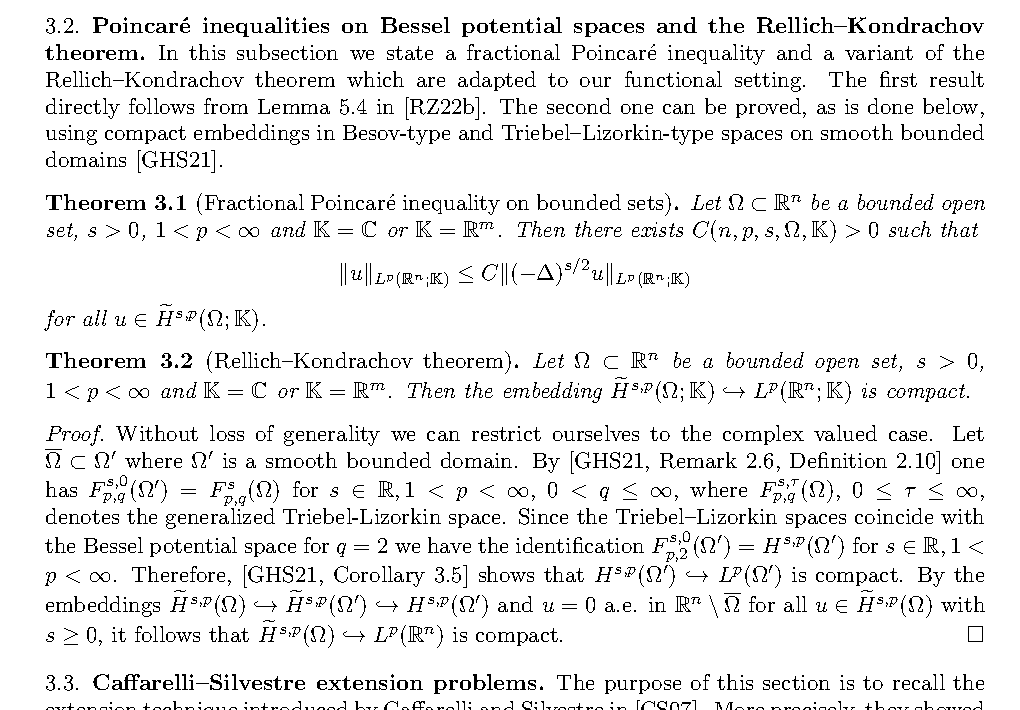
\includegraphics[width=0.93\linewidth]{figures/literature_theorem_crop.png}
\end{center}

A bounded search on 11--12 August 2026 checked the exact source title and
arXiv id, Question~7.4, the later theorem title, and combinations of
Bessel potential, fractional Poincar\'e, compact support, and endpoint
\(p=1\).  It recovered the source and the 2023 theorem but no explicit
endpoint result or full all-\(t\) answer.  The local run indexes contained
no duplicate.  Thus the \(1<p<\infty\) part is literature-known; the
endpoint and unified proof are candidate-new, pending specialist review.

\section*{Verification notes and limitations}

\begin{itemize}[leftmargin=*]
\item No reflexivity, weak compactness, Mikhlin theorem, or strong
\(L^1\) Riesz-transform bound is used.  Endpoint-sensitive steps use
finite-measure multipliers and Fr\'echet--Kolmogorov compactness.
\item The Fourier-support argument tests away from the origin, so it does
not assume that \(|\xi|^s\) is smooth at \(\xi=0\).
\item The \(K\)-dependent constant in Theorem~\ref{thm:main} is
existential.  Corollary~\ref{cor:classical} is quantitative for \(p>1\);
no \(P_1(\Omega)\)-formula is asserted.
\item The proof works for real or complex scalars and componentwise for
finite-dimensional targets.
\end{itemize}

\section*{Human-review recommendation}

Validity confidence is high.  Review the dyadic \(L^1\)-kernel bound, the
low/high asymptotics of the three radial symbols, and the endpoint
Fr\'echet--Kolmogorov step.  Novelty confidence is moderate because an
endpoint result may be hidden under harmonic-analysis terminology; author
and specialist citation review is recommended before publication claims.

\begin{thebibliography}{9}
\bibitem{source}
G.~Covi, K.~M\"onkk\"onen, and J.~Railo,
\emph{Unique continuation property and Poincar\'e inequality for higher
order fractional Laplacians with applications in inverse problems},
\href{https://arxiv.org/abs/2001.06210}{arXiv:2001.06210} (2020).

\bibitem{krz}
M.~Kar, J.~Railo, and P.~Zimmermann,
\emph{The fractional \(p\)-biharmonic systems: optimal Poincar\'e constants,
unique continuation and inverse problems},
\href{https://arxiv.org/abs/2208.09528}{arXiv:2208.09528};
Calc. Var. Partial Differential Equations 62 (2023).
\end{thebibliography}

\end{document}
